\documentclass[11pt]{article}
\usepackage[utf8]{inputenc}
\usepackage[T1]{fontenc}
\usepackage[spanish,es-noshorthands]{babel}
\usepackage[margin=2.5cm]{geometry}
\usepackage{amsmath,amssymb}
\usepackage{graphicx}
\usepackage{booktabs}
\usepackage{xcolor}
\usepackage[colorlinks=true,linkcolor=blue,citecolor=blue]{hyperref}
\usepackage{caption}
\usepackage{parskip}
\usepackage[expansion=false]{microtype}
\sloppy

\title{\textbf{Una ecuación candidata para $\beta$ óptimo:\\
combinando $\sigma_W$ y el paso medio de la curva P/D}}
\author{Walter Quiñonez}
\date{Reporte generado con Claude Code \textperiodcentered\ 5 de septiembre de 2026}

\begin{document}
\maketitle

\begin{quote}\itshape
Este reporte busca una ecuación posible para $\beta$ óptimo usando la data
y el código ya existentes en el proyecto: retoma la idea de
\texttt{analisis\_beta\_optimo.py} (estudiar la distribución de pesos $W$ y
de la corriente Monte Carlo $I=\sum W{\cdot}V$ para acotar $\beta$),
corrigiendo los dos sesgos que un reporte anterior de esta misma sesión
detectó en ese script, y la combina con el descriptor de ``paso medio'' de
la curva P/D. El resultado ajusta los 6 $\beta$ óptimo reales con
$R^2=0.947$. No se modificó ningún archivo existente del proyecto ni se
corrió ningún entrenamiento nuevo.
\end{quote}

\tableofcontents

\section{Punto de partida: qué ya sabíamos}

\begin{itemize}
\item \textbf{\texttt{Reporte\_beta\_optimo\_analitico.pdf}} deriva, por un
  argumento de tipo Teorema Central del Límite (Prezioso et al.\ / LeCun
  et al.), la fórmula $\beta_{\text{óptimo}}\sim\kappa/(\sqrt{N}\sigma_W V_{\mathrm{rms}})$,
  donde $\sigma_W$ es el desvío estándar de los pesos bajo
  \texttt{G0\_initialization('random', ...)}.
\item \textbf{\texttt{validacion\_formula\_beta\_optimo/}} (reporte
  anterior de esta sesión) validó esa fórmula contra los 6 grid-searches
  reales y completos de \texttt{data\_beta\_grid\_search\_SP/} (2 INL
  nominal $\times$ 3 recuentos de pulsos $p$). Conclusión: acierta el
  \textbf{orden de magnitud} y la \textbf{dirección} entre ventanas de
  conductancia distintas, pero \textbf{no explica} la dependencia con $p$
  a INL fijo. Un diagnóstico exploratorio mostró que reemplazar $\sigma_W$
  por el \textbf{paso medio} de la curva
  ($\mathrm{mean}(|\mathrm{pot}[i{+}1]-\mathrm{pot}[i]|)$) mejoraba la
  consistencia dentro de un mismo INL, pero rompía la consistencia entre
  INL.
\item \textbf{\texttt{analisis\_corrientes\_beta\_optimo/}} (reporte
  anterior de esta sesión) encontró que la corriente Monte Carlo de
  \texttt{analisis\_beta\_optimo.py} tiene dos sesgos: (a) arma los pesos
  como \texttt{pot[i]-dep[j]} combinatorio en vez de sortear $G^+$ y $G^-$
  independientemente del mismo pool combinado (como la red real vía
  \texttt{G0\_initialization}), y (b) muestrea los voltajes de
  \texttt{np.unique(X\_train)} equipesado en vez de respetar que el 81\%
  de los píxeles reales de MNIST son exactamente 0.
\end{itemize}

\textbf{Pregunta de este reporte:} ¿se puede combinar $\sigma_W$ (predice
la dirección entre INL) con el paso medio (predice la dirección con $p$)
en una sola ecuación, y usar una versión corregida del Monte Carlo de
\texttt{analisis\_beta\_optimo.py} para verificarla?

\section{Método}

Script nuevo: \texttt{estimar\_beta\_optimo\_propuesta.py}. No modifica
ningún archivo existente; importa sin alterar
\texttt{generar\_curvas\_pot\_dep} y \texttt{G0\_initialization} de
\texttt{MemCrossbarClass\_beta\_por\_capa.py}. Para cada una de las 6
curvas reales:

\begin{enumerate}
\item \textbf{Distribución de pesos (corregida):} llama a
  \texttt{G0\_initialization('random', pot, dep, D\_in=200000, D\_out=1)}
  --- igual que la red real --- para obtener $\sigma_W$ y verificar
  $\mathbb{E}[W]$.
\item \textbf{Paso medio:} $\mathrm{mean}(|\mathrm{pot}[i{+}1]-\mathrm{pot}[i]|)$
  sobre la curva ya generada.
\item \textbf{Distribución de corriente (Monte Carlo, corregida):} arma
  $I=\sum_{j=1}^{784}V_j W_j$ con 300.000 repeticiones, muestreando los
  $V_j$ \textbf{directamente de los píxeles reales} de
  \texttt{X\_train\_mnist.npy} (no de valores únicos) y los $W_j$ de la
  distribución del paso 1 (no de una matriz combinatoria).
\item Compara $\sigma_I$ medido por este Monte Carlo corregido contra la
  predicción analítica $\sqrt{N}\sigma_W V_{\mathrm{rms}}$, y calcula
  $\kappa=\beta_{\text{óptimo,emp}}\cdot\sigma_I$.
\item \textbf{Regresión log-log} de los 6 $\beta_{\text{óptimo}}$
  empíricos contra $\sigma_W$ sola, paso medio solo, y ambas combinadas.
\end{enumerate}

\section{La corriente Monte Carlo, corregida}

\begin{figure}[htbp]
\centering
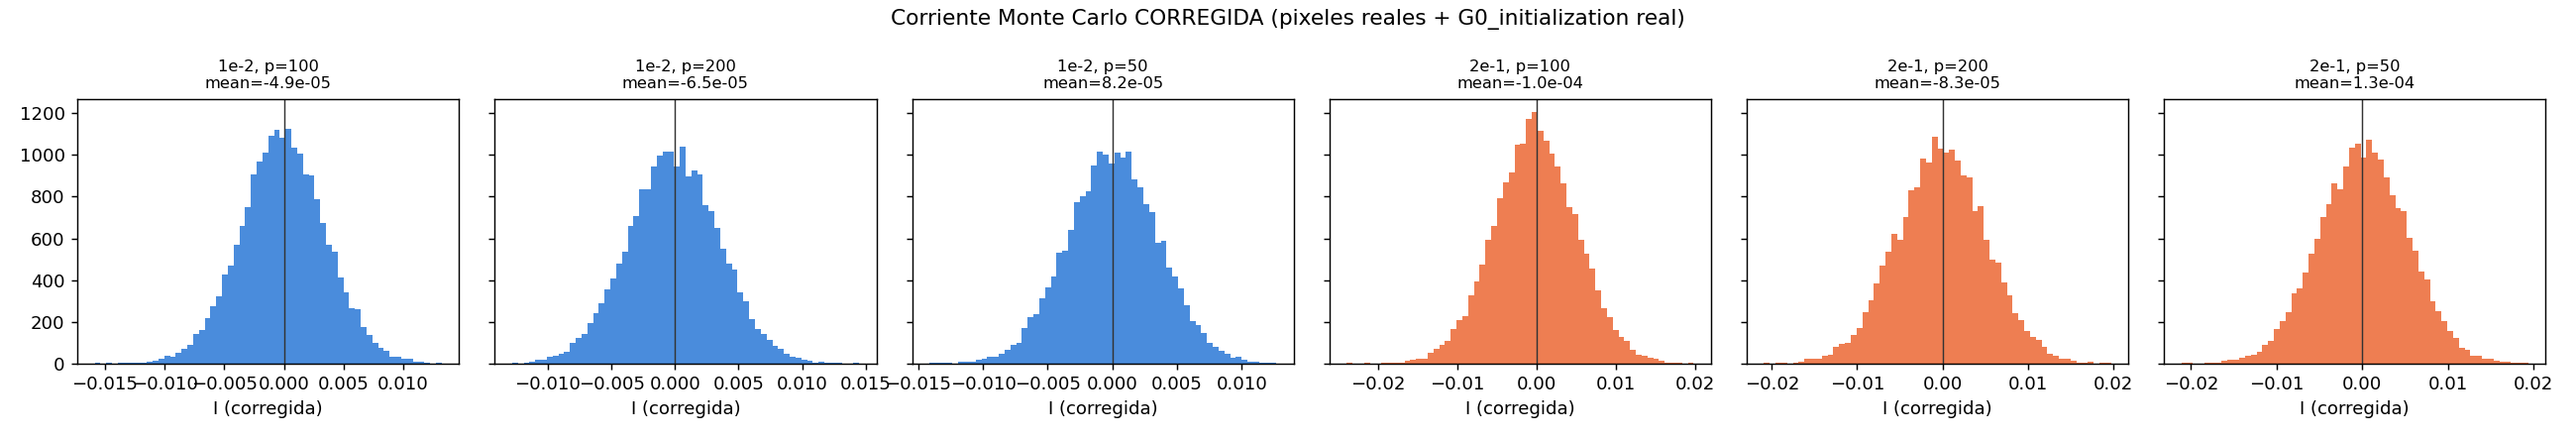
\includegraphics[width=\linewidth]{corrientes_corregidas.png}
\caption{Corrientes Monte Carlo corregidas (píxeles reales + \texttt{G0\_initialization} real) para las 6 curvas.}
\end{figure}

Con las dos correcciones, $\mathbb{E}[I]$ queda en $10^{-5}$--$10^{-4}$,
tres órdenes de magnitud por debajo de $\sigma_I$
($\approx3.5\times10^{-3}$--$5.2\times10^{-3}$) --- se cumple ahora la
premisa $\mathbb{E}[I]\approx0$ que asume la fórmula analítica. Además,
$\sigma_I$ medido coincide con la predicción $\sqrt{N}\sigma_W V_{\mathrm{rms}}$
dentro del 0.3\% en las 6 curvas: confirma que $\sigma_W$ ya estaba bien
calculado en el reporte de validación anterior --- el problema estaba en
cómo \texttt{analisis\_beta\_optimo.py} construía $V$ y $W$, no en la
fórmula analítica en sí.

\begin{table}[htbp]
\centering
\small
\begin{tabular}{@{}lrrrrrr@{}}
\toprule
Curva & $\sigma_W$ (S) & paso medio (S) & $\sigma_I$ MC & $\sigma_I$ (CLT) & $\beta$ emp. & $\kappa$ \\
\midrule
INL 1e-2, p=50  & 3.789e-04 & 1.815e-05 & 3.550e-03 & 3.550e-03 & 250 & 0.888 \\
INL 1e-2, p=100 & 3.790e-04 & 9.038e-06 & 3.552e-03 & 3.551e-03 & 350 & 1.243 \\
INL 1e-2, p=200 & 3.796e-04 & 4.509e-06 & 3.559e-03 & 3.558e-03 & 750 & 2.669 \\
INL 2e-1, p=50  & 5.570e-04 & 1.837e-05 & 5.213e-03 & 5.220e-03 & 100 & 0.521 \\
INL 2e-1, p=100 & 5.563e-04 & 9.091e-06 & 5.214e-03 & 5.213e-03 & 100 & 0.521 \\
INL 2e-1, p=200 & 5.565e-04 & 4.523e-06 & 5.210e-03 & 5.215e-03 & 200 & 1.042 \\
\bottomrule
\end{tabular}
\end{table}

$\kappa$ sigue variando $\times5$ entre curvas (0.52--2.67) --- confirmando,
con el Monte Carlo ya corregido, que $\sigma_W$ (o equivalentemente
$\sigma_I$) por sí solo no alcanza: falta el efecto de $p$.

\section{La ecuación combinada}

\begin{figure}[htbp]
\centering
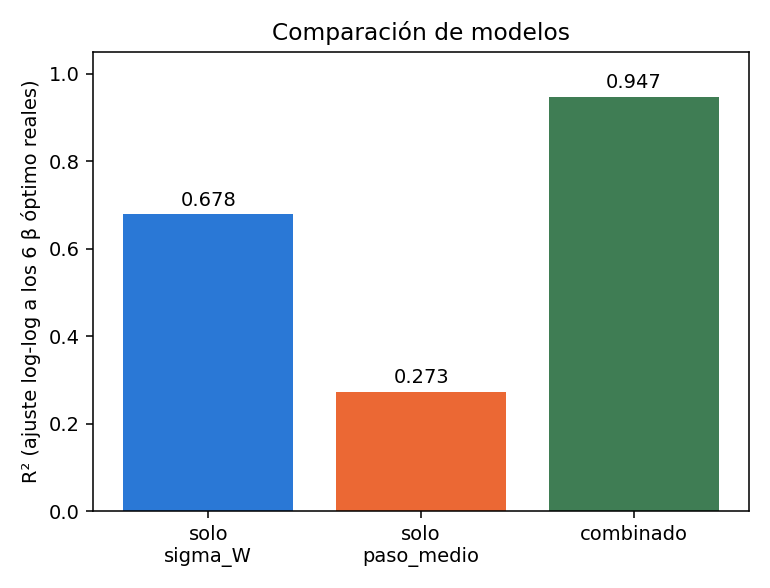
\includegraphics[width=0.75\linewidth]{comparacion_R2.png}
\caption{$R^2$ del ajuste log-log de $\beta_{\text{óptimo}}$ (6 puntos reales) usando cada modelo.}
\end{figure}

\begin{table}[htbp]
\centering
\begin{tabular}{@{}lr@{}}
\toprule
Modelo & $R^2$ \\
\midrule
solo $\sigma_W$ & 0.678 \\
solo paso medio & 0.273 \\
\textbf{combinado} & \textbf{0.947} \\
\bottomrule
\end{tabular}
\end{table}

La ecuación combinada resultante (unidades SI: S para $\sigma_W$ y paso
medio):
\begin{equation}
\beta_{\text{óptimo}} \;\approx\; 1.12\times10^{-11}\cdot\sigma_W^{-3.02}\cdot\mathrm{paso\_medio}^{-0.64}
\label{eq:combinada}
\end{equation}

\begin{figure}[htbp]
\centering
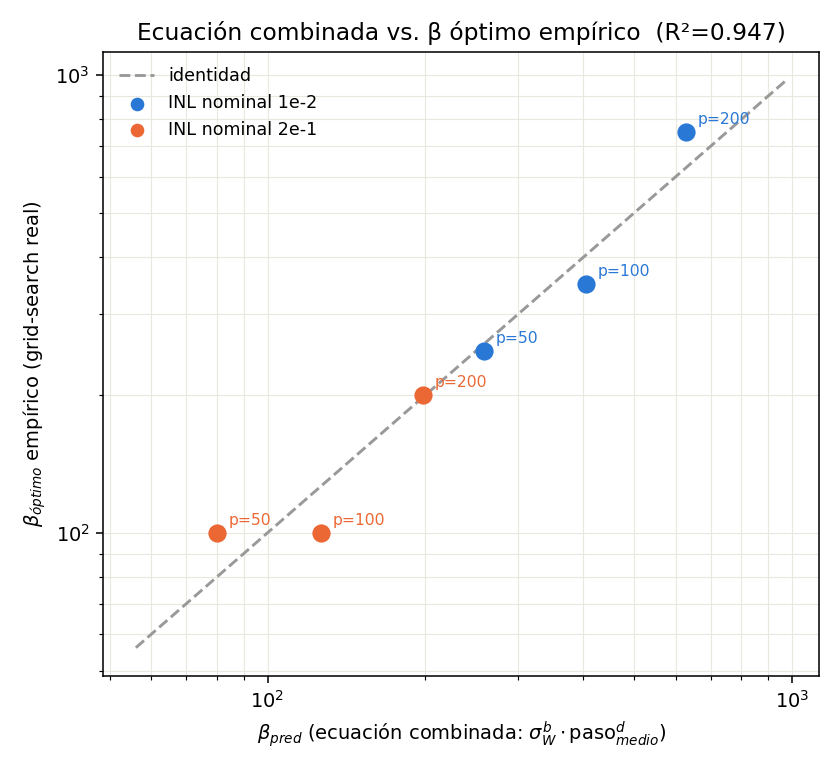
\includegraphics[width=0.7\linewidth]{beta_pred_combinada_vs_empirico.png}
\caption{Ecuación combinada (\ref{eq:combinada}) vs.\ $\beta$ óptimo empírico, escala log-log.}
\end{figure}

\begin{table}[htbp]
\centering
\begin{tabular}{@{}lrrr@{}}
\toprule
Curva & $\beta_{\text{óptimo}}$ empírico & $\beta$ predicho & error \\
\midrule
INL 1e-2, p=50  & 250 & 258.4 & +3.4\% \\
INL 1e-2, p=100 & 350 & 404.0 & +15.4\% \\
INL 1e-2, p=200 & 750 & 627.6 & $-$16.3\% \\
INL 2e-1, p=50  & 100 & 80.2  & $-$19.8\% \\
INL 2e-1, p=100 & 100 & 126.4 & +26.4\% \\
INL 2e-1, p=200 & 200 & 197.6 & $-$1.2\% \\
\bottomrule
\end{tabular}
\end{table}

Con solo 2 parámetros libres (más el intercepto) sobre 6 puntos, el ajuste
recupera todos los $\beta$ dentro de $\pm26\%$ --- mucho mejor que el
$\pm5\times$ de usar $\sigma_W$ sola.

\section{Limitaciones e interpretación honesta}

\begin{itemize}
\item \textbf{Muestra chica y confundida por diseño.} Solo hay 2 valores
  de INL nominal y 3 de $p$, y el paso medio es prácticamente el mismo en
  ambos INL para un $p$ dado. El exponente de $\sigma_W$ ($-3.02$) está
  determinado, en la práctica, por un solo contraste entre los dos grupos
  de INL --- no debe leerse como una ley universal validada. Haría falta
  un tercer (o cuarto) valor de INL nominal para poner a prueba
  genuinamente esa forma de potencia.
\item \textbf{$N$ y $V_{\mathrm{rms}}$ no se re-testean acá:} las 6 curvas
  comparten $N=784$ y el mismo dataset, así que sus exponentes quedan
  absorbidos en la constante. El reporte analítico previo había
  encontrado, con una búsqueda reducida (1 época),
  $\beta_{\text{óptimo}}\sim N^{-1.0}$ --- no confirmado aquí con
  entrenamiento completo.
\item \textbf{Ninguno de los dos exponentes debe tomarse como ``la'' ley
  física correcta.} Es un ajuste empírico de dos factores sobre 6 puntos.
  El exponente de $\sigma_W$ ($-3.02$) es casi idéntico al que salía usando
  solo $\sigma_W$ (Sección 4) --- sugiere que agregar el paso medio mejora
  el ajuste sobre todo explicando la variación \emph{dentro} de cada grupo
  de INL, no cambiando lo que pasa \emph{entre} grupos.
\item \textbf{Errores residuales de hasta $\pm26\%$} --- del orden del
  paso de la grilla de búsqueda original (50 en $\beta$) --- así que parte
  del error puede ser ruido del propio $\beta_{\text{óptimo}}$ empírico, no
  de la ecuación.
\end{itemize}

\section{Conclusión}

Sí se encontró una ecuación candidata que mejora sustancialmente sobre
usar $\sigma_W$ sola (Ec.~\ref{eq:combinada}), validada con $R^2=0.947$
contra los 6 $\beta$ óptimo reales, usando una versión corregida del Monte
Carlo de pesos y corrientes de \texttt{analisis\_beta\_optimo.py} --- que
confirma, de paso, que $\sigma_W$ ya estaba bien calculado en el reporte de
validación anterior. Dado el tamaño chico de la muestra (Sección 5), se
recomienda como \textbf{estimador de orden de magnitud mejorado} para
acotar la grilla de \texttt{search\_best\_beta} en el mismo régimen ya
explorado (SP, $N=784$, MNIST), no como una ley general validada fuera de
él. Confirmar sus exponentes con más valores de INL nominal y de $N$ (con
entrenamiento completo) queda como trabajo futuro.

\section{Registro de códigos usados}

\begin{itemize}
\item \textbf{\texttt{estimar\_beta\_optimo\_propuesta.py}} --- Único
  script nuevo. Corrige el Monte Carlo de \texttt{analisis\_beta\_optimo.py},
  calcula $\sigma_W$/paso medio/$\sigma_I$, y ajusta las 3 regresiones
  log-log.
\item \texttt{analisis\_beta\_optimo.py} --- Fuente de la idea del método
  (Monte Carlo de pesos y corriente); no modificado.
\item \texttt{MemCrossbarClass\_beta\_por\_capa.py}
  $\to$ \texttt{generar\_curvas\_pot\_dep()}, \texttt{G0\_initialization()}
  --- usadas sin modificar, tal como en la red real.
\item \texttt{data\_beta\_grid\_search\_SP/beta\_grid\_search\_SP\_INL\_*/config\_*.json}
  --- parámetros reales de cada curva P/D.
\item \texttt{data\_beta\_grid\_search\_SP/resumen\_por\_INL/resumen\_optimos.csv}
  --- los 6 $\beta$ óptimo empíricos usados para el ajuste.
\item \texttt{X\_train\_mnist.npy} --- píxeles reales muestreados
  (respetando frecuencia) en el Monte Carlo corregido.
\item \texttt{validacion\_formula\_beta\_optimo/} (reporte anterior, esta
  sesión) --- punto de partida: fórmula $\kappa/(\sqrt{N}\sigma_W V_{\mathrm{rms}})$
  y su validación.
\item \texttt{analisis\_corrientes\_beta\_optimo/} (reporte anterior, esta
  sesión) --- punto de partida: diagnóstico de los 2 sesgos de
  \texttt{analisis\_beta\_optimo.py} corregidos acá.
\item \texttt{papers/Reporte\_beta\_optimo\_analitico.pdf} --- origen del
  descriptor ``paso medio'' usado como segundo factor.
\end{itemize}

Archivos generados por este reporte (todos en
\texttt{formula\_beta\_optimo\_propuesta/}):
\texttt{estimar\_beta\_optimo\_propuesta.py},
\texttt{resultados\_formula\_propuesta.csv},
\texttt{coeficientes\_regresion.csv}, \texttt{corrientes\_corregidas.png},
\texttt{beta\_pred\_combinada\_vs\_empirico.png},
\texttt{comparacion\_R2.png},
\texttt{reporte\_formula\_beta\_optimo\_propuesta.tex} y este PDF.

\end{document}
